\documentclass{document_layout}

% Title and author information 
\title{PHOTON COINCIDENCE MEASUREMENTS}
\author{
    Eduardo Barroso\address{1} \quad Eikin Kizilkan\address{1} \quad Utku Karaca \address{2} \\[1em]
    \address{1} \textit{École Polytechnique Fédérale de Lausanne (EPFL)} \\
    \address{2} \textit{Novoviz}
}
\date{\today}

%Abstract 
\setabstract{
This work presents a brief characterization of SPADs and their application in correlation measurements.
Measurements using lasers, thermal and pseudothermal light sources were performed to understand the limitations of measuring second order coherence.
Initial measurements yield the zero-delay coherence value $g^{(2)}(0)$ for pulsed lasers and map the complete correlation function  $g^{(2)}(\tau)$. 
Finally, a rotating diffuser was implemented to generate dynamic speckle patterns providing a demonstration of speckle decorrelation time ($\tau_c$). 
}

% Begin the document
\begin{document}

\maketitle

\section*{Introduction}
\addcontentsline{toc}{section}{Introduction}
\input{Sections/introduction}

\newpage
\onecolumn
\tableofcontents
\twocolumn

\newpage
\section*{Equipment and Materials}
\addcontentsline{toc}{section}{Equipment and Materials}
%\subsection*{Facilities}
% \begin{center}
%     \begin{tabular}{ |c|c|c| }
%         \hline
%         Room      &  Description &  Notes     \\
%         MC A3 153 &  Optics Lab    &  CW       \\
%         %MC A3 193 & Rad/Optics Lab & Pulsed Laser \\
%         \hline
%     \end{tabular}
% \end{center}


\subsection*{Lasers and Light Sources}
\begin{itemize}
    \item Pulsed LASER:  PicoQuant PDL Series
    \begin{itemize}\footnotesize
        \item \textbf{PicoQuant Laser Diode Head}
        \item \textbf{Wavelength:} 640 nm
        \item \textbf{Repetition Rate ($f_{rep}$):} Tunable frequencies (operated between 1 MHz and 80 MHz).
    \end{itemize}
    
    \item \textbf{Continuous Wave (CW) LASER 1}
    \begin{itemize}\footnotesize
       \item \textbf{Thorlabs S1FC660 (Fiber-coupled)}
       \item \textbf{Wavelength:} 660 nm
       \item \textbf{Power:} Tunable from 0 mW to 19.8 mW
    \end{itemize}

    \item \textbf{Continuous Wave (CW) LASER 2}
    \begin{itemize}\footnotesize
        \item Thorlabs Benchtop Laser Diode Controller with mounted laser diode head.
        \item \textbf{Wavelength:} 785 nm
        \item \textbf{Power:} Tunable diode current (between 62.7 mA and 65.5 mA)
    \end{itemize}

    \item \textbf{Pseudothermal Light Simulator}
    \begin{itemize}\footnotesize
        \item Rotating glass diffuser (K10CR1/M). Motor Speed up to $20^\circ /s$. 
        \item Continuous Wave (CW) LASER 2
    \end{itemize}
\end{itemize}

\subsection*{Timing Electronics}
\begin{itemize}
    \item Swabian Instruments Time Tagger
    \begin{itemize}\footnotesize
        \item \href{https://www.swabianinstruments.com/static/documentation/TimeTagger/}{Model: Ultra, USB 3.0}
        \item Max Data Transfer Rate: 90 MTags/s
        \item Max Input Frequency: 475 MHz
        \item Dead Time: 2.1 ns
        \item Base Jitter: \href{https://www.swabianinstruments.com/static/downloads/TimeTaggerSeries.pdf}{42 ps RMS (100 ps FWHM)}
        \item Trigger Level Range: -2.5 V to +2.5 V
    \end{itemize}
    
\end{itemize}

\subsection*{Detectors and Optical Components}
\begin{itemize}
    \item \textbf{2 Pixel SPAD Module}
    \begin{itemize}\footnotesize
        \item Model: \href{https://novoviz.com/two-pixel-correlator/}{NV02TPX}
        \item 64 bins of up to $5 ns$ width
    \end{itemize}

    \item \textbf{Linear SPAD Array Module}
    \begin{itemize}\footnotesize
        \item \textbf{Model:} \href{https://novoviz.com/small-line/}{Novoviz Small Line Sensor}
        \item \textbf{Architecture:} 24-pixel linear SPAD array
    \end{itemize}
    
    \item \textbf{Neutral Density Filters}: 0.6, 2.3
\end{itemize} 

\newpage
\section*{Layout and Calibration}
\addcontentsline{toc}{section}{Layout and Hardware Calibration}
The experimental layout used throught the measurements is presented figure \ref{fig:exp_lay}. 
The layout is designed to allow interchanging light sources incident on the SPAD. 
Optical elements can also be introduced between the source and the SPAD for attenuation, modulation and alignment purposes.\\   

\begin{figure}[htpb]
    \centering
    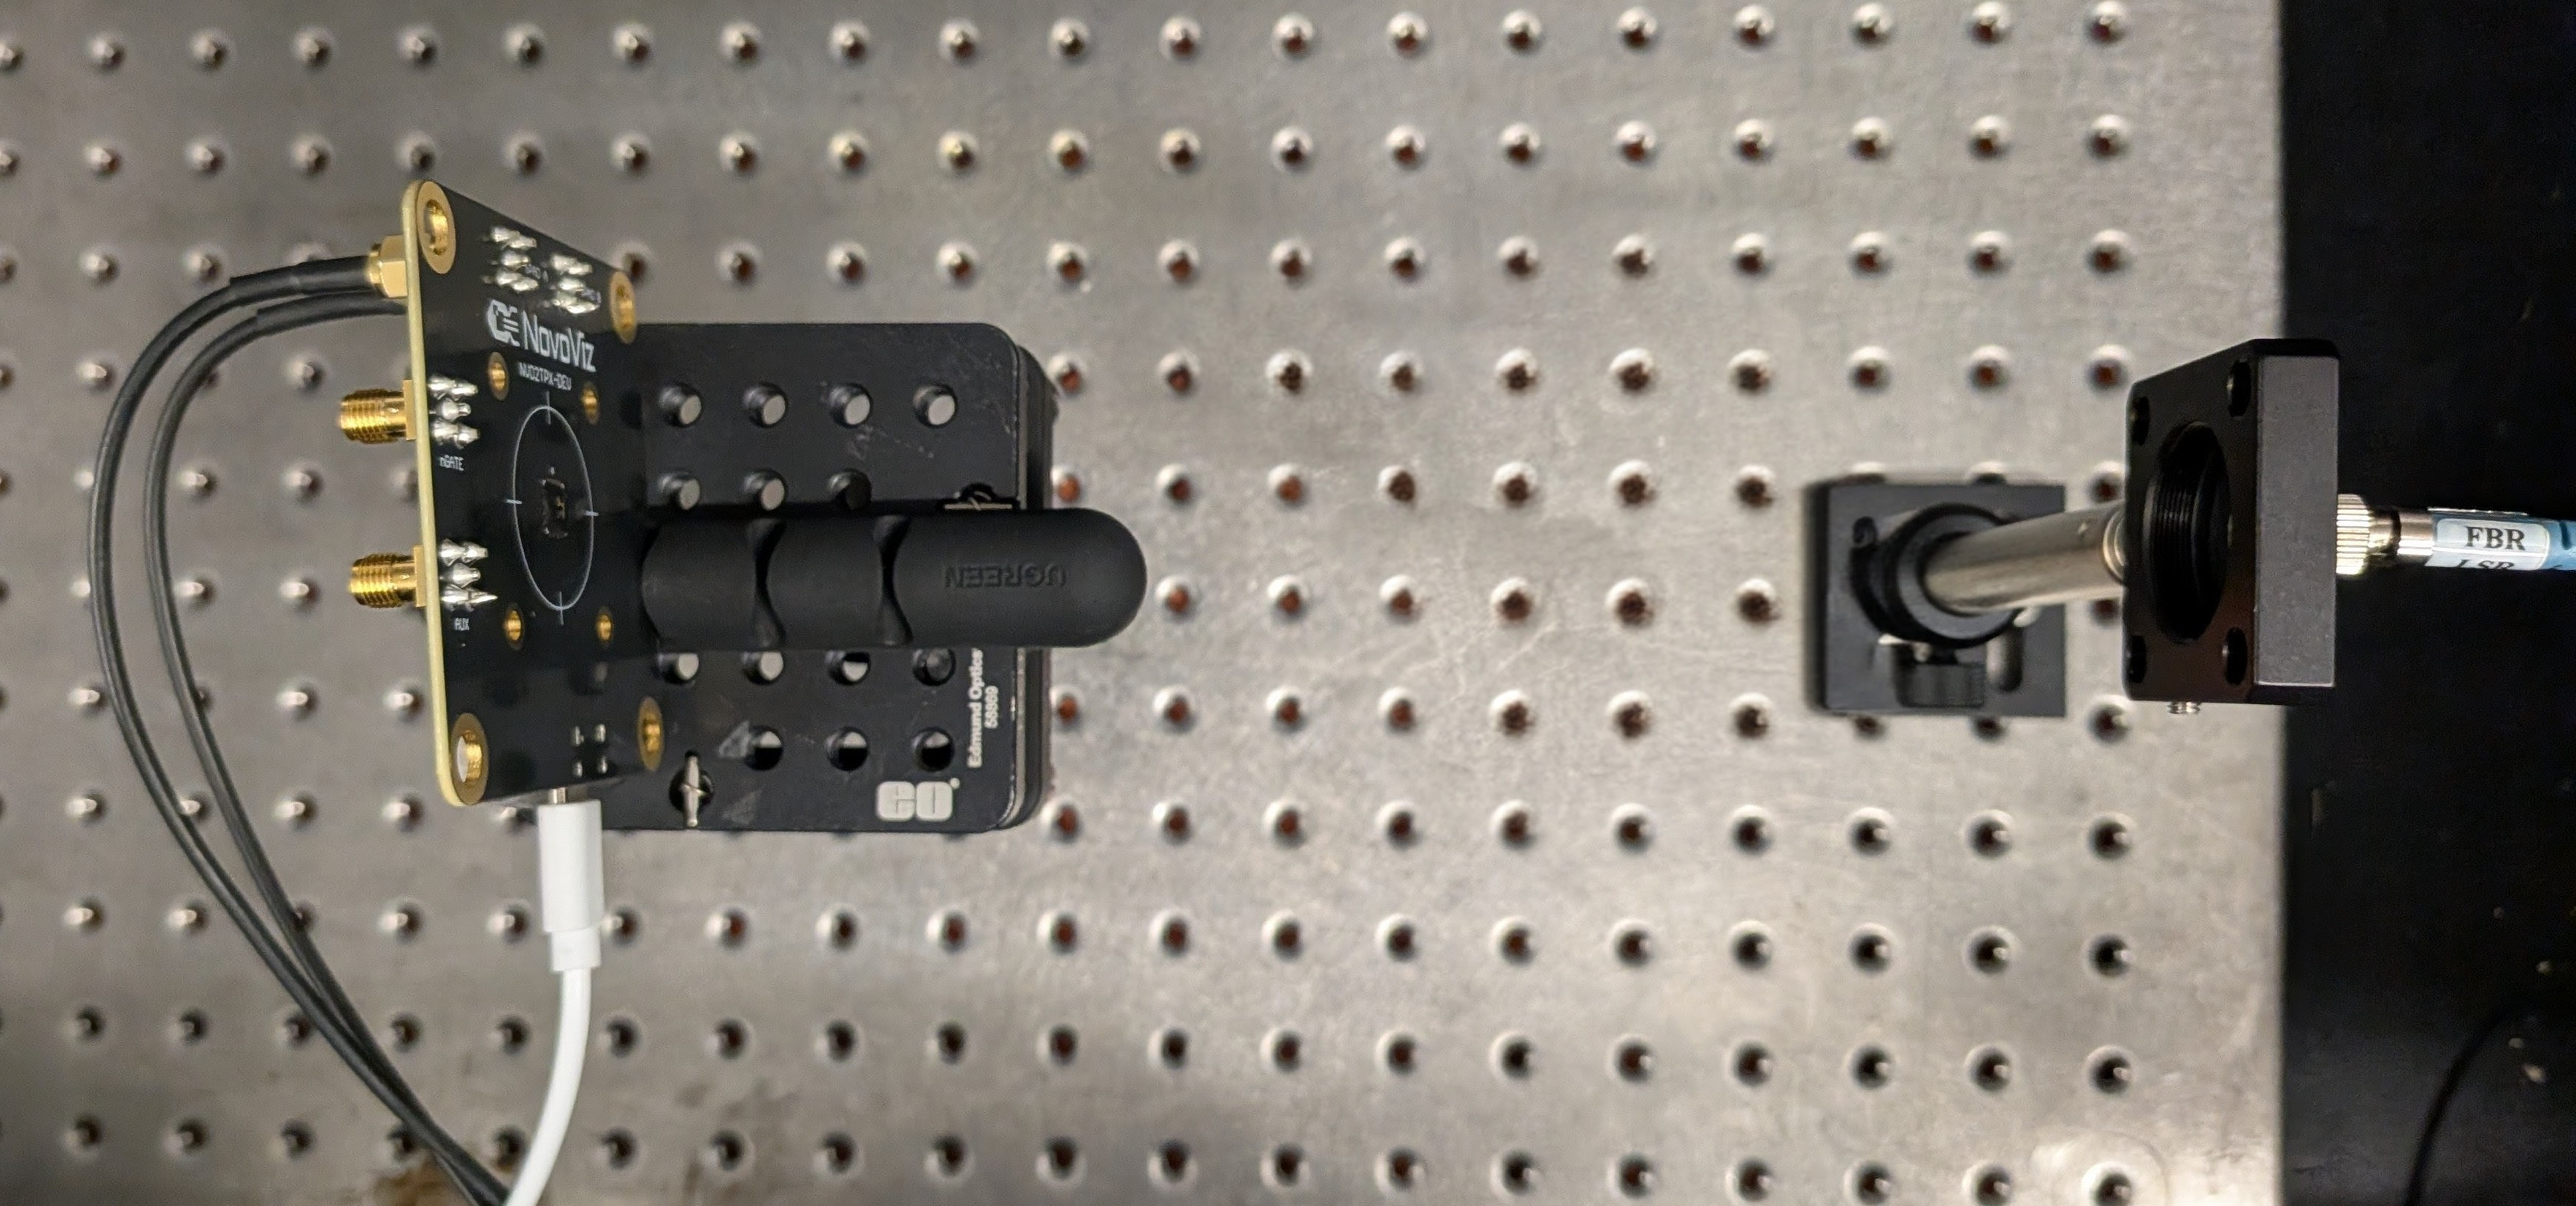
\includegraphics[width=0.45\textwidth]{Figures/exp_layout_plain.jpg}
    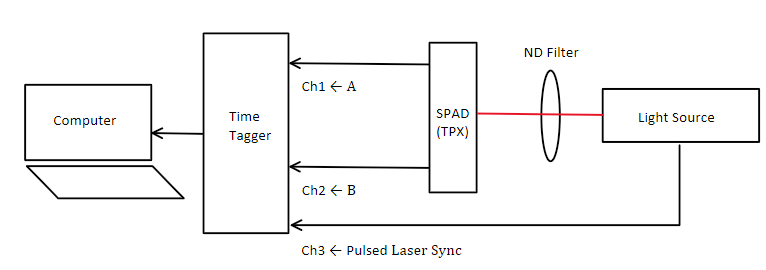
\includegraphics[width=0.45\textwidth]{Figures/exp_layout1_diagram.png}
    \caption{Experimental layout. Source is feed into the system with fiber optic cable that couples into free space with the \href{https://www.thorlabs.com/item/SM1FC2}{SM1 FC2} and irradiates the SPAD.}
    \label{fig:exp_lay}
\end{figure}

\subsection{TDC Application Programming Interface}
To process the timestamps generated by the single-photon detectors, this work utilizes the Swabian Instruments Time Tagger API \cite{swabian_correlation_web}, specifically the \href{https://www.swabianinstruments.com/static/documentation/TimeTagger/api/measurements/time_histograms.html#_CPPv411Correlation}{\texttt{tt.Correlation}} class. 
This function computes the cross-correlation between two detection channels. 

The algorithm operates within a user-defined correlation time window. 
This window is determined by specifying a temporal \texttt{bin width} and a total \texttt{number of bins}. 
For every photon event registered on a start channel, the algorithm calculates the time delay ($\tau$) to subsequent events on a stop channel, provided those events fall within the bounded correlation window. 
These computed delays are continuously accumulated and sorted into their respective time bins resulting in the final coincidence histogram, which is directly proportional to the second-order coherence function, $g^{(2)}(\tau)$.

\subsection{SPAD Characterization}
With the set up complete, a SPAD calibration is performed to verify the setup is operating within the expected margins. 
With an autocorrelation measurement we expect to extract a value for the dead time of the detector, and the afterpulsing probability and confirm that the digital pipeline is working as expected. 
The autocorrelation is measured with the \texttt{tt.Correlation} function with the same SPAD as the start and stop channel. 
The procedure is listed bellow: 
\begin{enumerate}
    \item Connect the CW laser source 1 to the fiber optics line feeding the system. 
    \item Connect the SPAD detectors with SMA Cables to Swabian Time Tagger. 
    \item Initialize the autocorrelation measurement (\texttt{tt.Correlation}) using a single SPAD channel as both the "start" and "stop" trigger. 
    \item Wait for detection events to accumulate for 10 seconds.
    \item Extract dead time and afterpulsing probabilities from data (See figure \ref{fig:autocorr}).
    \item Repeat 5 times to gather statistics. 
\end{enumerate}

\begin{figure}[htpb]
    \centering
    %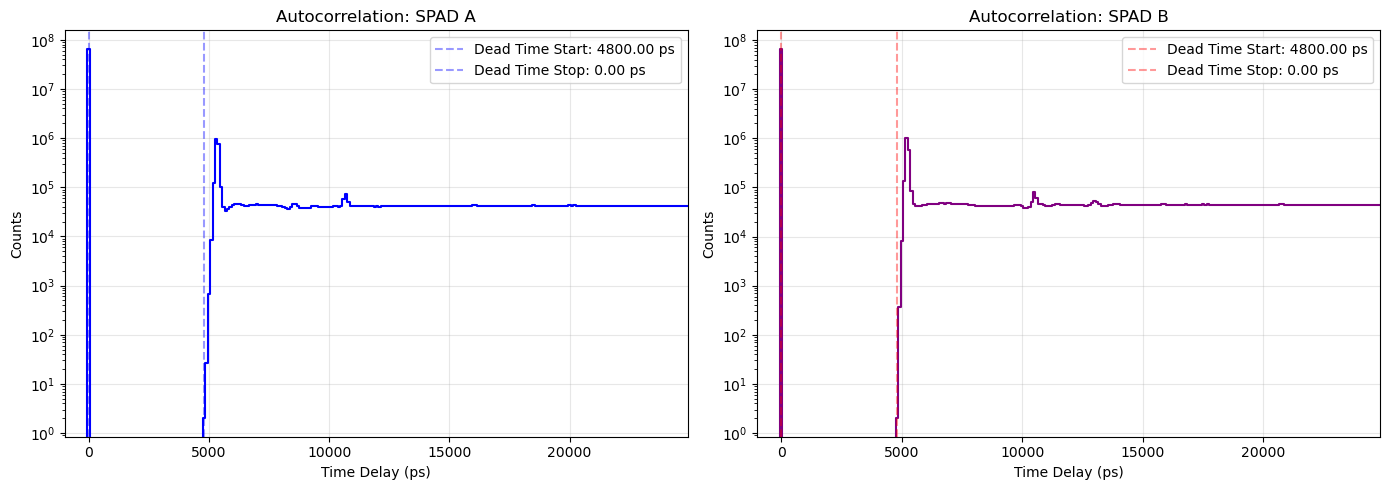
\includegraphics[width=0.5\textwidth]{Figures/autocorr_measurement.png}
    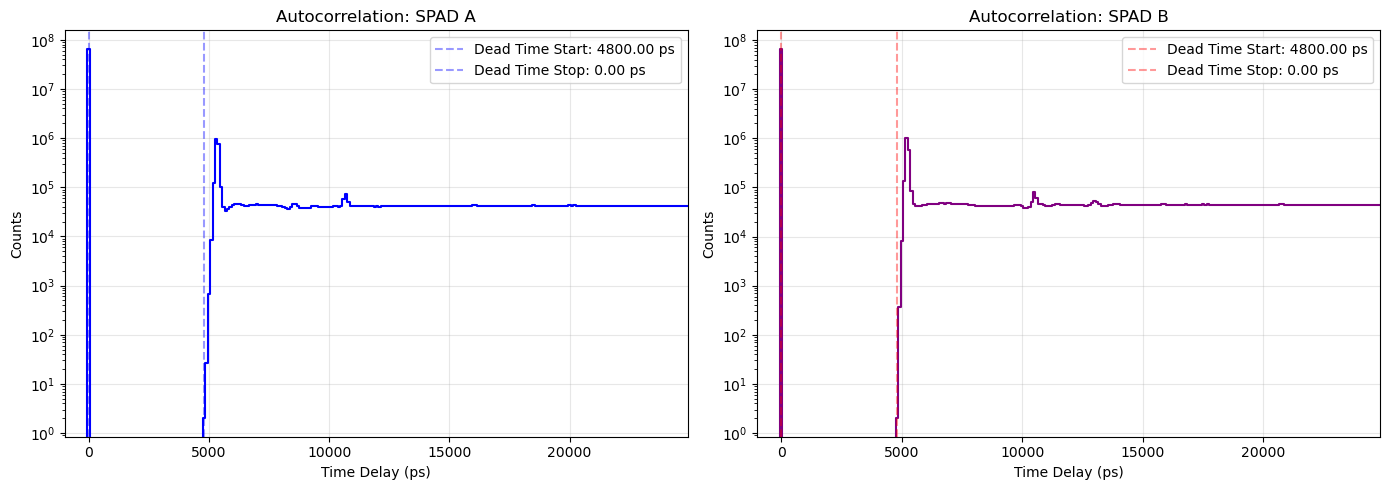
\includegraphics[trim=0cm 0cm 17.4cm 0cm, clip, width=\linewidth]{Figures/autocorr_measurement.png}
    \caption{Autocorrelation histogram of the SPAD channel 1. The measurement was taken with an illumination count rate of 10 Mcps and a histogram bin width of 100 ps.}
    \label{fig:autocorr}
\end{figure}

Figure \ref{fig:autocorr} shows the resulting autocorrelation histogram. 
The dead time is quantitatively defined as the temporal delay at which the coincidence counts recover from 0 counts. 
To calculate the afterpulsing probability ($P_{ap}$), the steady-state baseline counts are first estimated from the flat region of the histogram occurring well after the detector recovery. 
This baseline is subtracted from the total counts to isolate the excess detections. $P_{ap}$ is then determined by integrating these excess counts from the end of the dead time ($t_{dt}$) to the end of the time window ($t_{end}$), normalized by the total number of valid trigger events ($N_{triggers}$):

\begin{equation}
    P_{ap} = \frac{\sum_{t = t_{dt}}^{t_{end}} (N_{counts}(t) - N_{baseline})}{N_{triggers}}
\end{equation}

The results of this characterization are summarized in Table \ref{tab:calibration_summary}.

\begin{table}[htpb]
    \centering
    \caption{Summary of Detector Calibration Parameters}
    \label{tab:calibration_summary}
    \resizebox{\linewidth}{!}{%
    \begin{tabular}{lcc}
        \toprule
        \textbf{Parameter} & \textbf{SPAD 1} & \textbf{SPAD 2} \\
        \midrule
        %DCR (cps) & $9.74 cps$ & $10,301.49$ \\
        Mean Dead Time (ns) & $4.90 \pm 0.12$ & $4.85 \pm 0.09$ \\
        Maximum Repetiton Rate (MHz) & 204.08 & 206.19 \\
        Afterpulsing Probability (\%) & 2.41 & 2.30 \\
        \bottomrule
    \end{tabular}
    }
\end{table}


%\newpage
\section*{Poissonian Statistics Verification}
\addcontentsline{toc}{section}{Poissonian Statistics Verification}
\subsection{Coherent Light}

This section presents the experimental measurement of photon count distributions, which are used to infer Poissonian and super-Poissonian statistics.
Measurements were performed using the CW laser 1 (listed in section \ref{sec:lightsources}) in the following manner. 

\begin{itemize}
    \item Feed the CW laser 1 into the optical setup in figure \ref{fig:exp_lay}. 
    \item Mount Filter in between the source and the SPAD. 
    \item Set the integration time window to $100 \hspace{1mm} \mu s$ 
    \item Connect SPAD to Swabian Time Tagger. 
    \item Run the \texttt{tt.Counter} function and plot histogram. 
\end{itemize}

\begin{figure}[htpb]
    \centering
     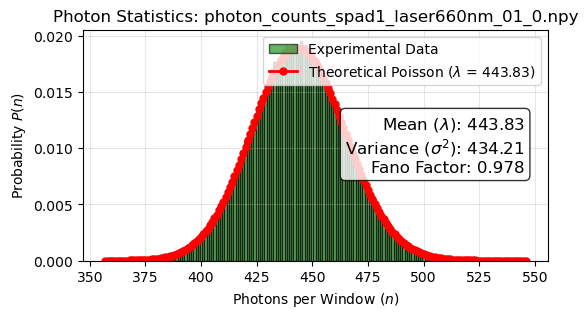
\includegraphics[width=0.5\textwidth]{Figures/photon_counts_spad1_01_0.png}
    \caption{Photon count distribution ($1 mW$).}
    \label{fig:photon_counts_spad1_01_0}
\end{figure}

\begin{figure}[htpb]
    \centering
     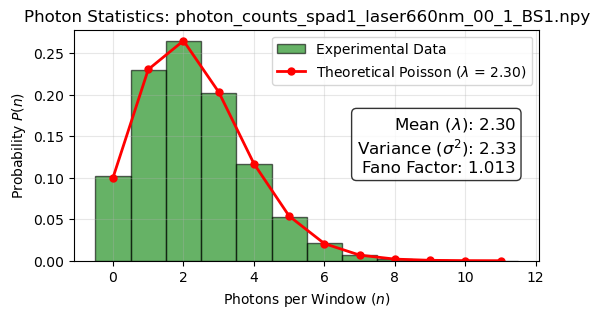
\includegraphics[width=0.5\textwidth]{Figures/photon_counts_spad1_00_1.png}
    %\rule{0.5\textwidth}{5cm}
    \caption{Photon count distribution($0.1 mW$).}
    \label{fig:photon_counts_spad1_00_1}
\end{figure}


As shown in Figure \ref{fig:photon_counts_spad1_00_1}, the coherent laser source yields a Poissonian distribution even as we vary the power of the CW laser.
Furthermore, in Figure \ref{fig:photon_counts_spad1_01_0}, a polarizing beam splitter was introduced to measure the curve in the low-power regime, also resulting in a Poissonian distribution.
The fact that the variance closely matches the mean ($\sigma^2 \approx \mu$) is consistent with the expected Poissonian statistics of coherent laser light. \\

\subsection{Non-Coherent Light}
We then replaced the light source with a fluorescent light bulb, acting as a non-coherent broadband source, and ran the previous experiment with the CW laser turned off. 
The resulting super-Poissonian distribution is shown in Figure \ref{fig:photon_counts_spad1_lablight}.

\begin{figure}[htpb]
    \centering
    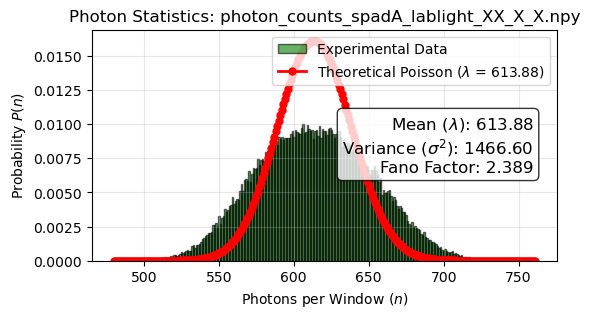
\includegraphics[width=0.5\textwidth]{Figures/photon_counts_spad1_lablight.png}
    %\rule{0.5\textwidth}{5cm}
    \caption{Photon counting statistics of the fluorescent light bulb, utilized here as a non-coherent broadband source. The experimental data follows a super-Poissonian distribution.}
    \label{fig:photon_counts_spad1_lablight}
\end{figure}


\newpage
\section*{Coincidence Measurements}
\addcontentsline{toc}{section}{Coincidence Measurements}
\input{Sections/exp_coincidences.tex}

\newpage 
\onecolumn
\section*{Conclusion}
\addcontentsline{toc}{section}{Conclusion}
This work demonstrated the use of single-photon avalanche diodes (SPADs) and time-correlated single-photon counting (TCSPC) to measure the second-order correlation function, $g^{(2)}(\tau)$, of various light sources. 
By characterizing the detector hardware, the fundamental limitations of the measurements were established, and the statistical signatures of coherent lasers and super-Poissonian sources were obtained. \\

An experimental data-processing pipeline was successfully implemented and validated for cross-correlation measurements.
For pulsed laser illumination, the zero-delay cross-correlation, $g^{(2)}(0)$, was successfully measured by varying the coincidence criterion and under both high and low count-rate conditions, demonstrating the critical impact of statistical precision. 
Furthermore, mapping the full temporal correlation function, $g^{(2)}(\tau)$, successfully resolved the characteristic comb structure of the pulsed emission. 
By adjusting the correlation bin width to match the laser period, the expected flat integration baseline was recovered, validating the pipeline's capability to accurately capture and process cross-correlation dynamics. \\

The measurement of a non-coherent broadband source (fluorescent lab light) highlighted the temporal limits of the detector architecture. 
The femtosecond decorrelation times of such broad-bandwidth sources were shown to be entirely averaged out by the finite timing resolution of the SPADs and readout electronics. 
The residual signal observed at zero delay was attributed to electronic timing effects and optical crosstalk between adjacent pixels, rather than true quantum photon bunching. \\

Finally, a proof-of-principle demonstration of Diffuse Correlation Spectroscopy (DCS) was implemented using a rotating diffuser phantom. 
Scattering a continuous-wave laser through this dynamic medium generated macroscopic speckle intensity fluctuations in the millisecond regime. 
This allowed the TCSPC hardware to accurately capture the exponential decorrelation of the dynamic speckle pattern.
Furthermore, using the linear SPAD array through multi-pixel spatial averaging proved effective in reducing baseline measurement noise in accordance with the theoretical $1/\sqrt{N}$ scaling. 
Ultimately, this methodology captured the dynamic photon statistics, accounted for detector artifacts, and linked the extracted decorrelation times to the kinematic properties of the macroscopic target.
\twocolumn

% References
\onecolumn
\printbibliography
\addcontentsline{toc}{section}{References}
\twocolumn

%\onecolumn
%\newpage
%\section*{Questions}
%\begin{itemize}
    \item 1- Your jitter curves here are different than what you have presented in the final presentation or other slides you have sent me. What changed? 
    \item 1A- In the presentation, I showed a $425 ps$ of FWHM corresponding to the pulsed laser operating at $1MHz$ and $33 \mu W$. On the report opted to show a $160 ps$ FWHM at $80MHz$ and $33 \mu W$ . I saved all the data in: \verb|datacoincidence_meas_run1_80MHz_100uW| and \verb|data_coincidence_meas_run2_1MHz_33uW|. I also have saved values for if you are intrested in exporing these results. I also have: \verb|data_coincidence_meas_run1_1MHz_3uW| and \verb|data_coincidence_meas_run1_ThermalSources_g2|. I placed the two figures bellow for referece. In my opinion, this is due to the source jitter rather than the SPAD. 
    \item 2- These look better, but how did you get these, whats the difference? 
    \item 2A- Both the power and the frequency changed. Although I suspect the frequency is the main culpit. Longer jitter corresponded to the setting with lower frequency. 
    \item 3- Important for full Coincidence Measurements section!: I believe you did the same mistake
here as during your final presentation. You should have used two SPADs in this
experiment, as written in the procedures I gave you in the beginning. Therefore,
there is no auto-correlation, there is no term of auto-correlation function for
laser or thermal lamp etc. here. It is still cross-correlation. You should have
built a histogram based on timestamps between two SPAD channels, not with
the laser. As I wrote in the presentation, there is no laser sync used here. Or, I
am very confused with the experiment you performed here. You switched to
getting auto-correlation of single SPADs (not laser) with rotating diffuser
experiment. You utilized SPADA and SPADB until that experiment, which makes
your results cross-correlation until rotating diffuser. 
\item 3A-You are entirely correct —the measurements were \textbf{cross-correlations} between the two SPADs, not autocorrelations. I had the Wiener-Khinchin theorem on my mind from my recent metrology exam and mixed up the terminology in the text. I proceed to clarify this mistake with the actual syntax I used for the measurements:
\begin{itemize} \footnotesize
    \item For the 1st Measurement, I measured cross-correlation: 
    \item[] $counter = tt.Counter(tagger, [spadA, spadB, sync], binwidth=exposuretime, nvalues=1) $
    \item[] $coinc = tt.Coincidence(tagger, [spadA, spadB], coincidencewindow) $
    \item[] $coinccounter = tt.Counter(tagger, [coinc.getChannel()], binwidth=exposuretime, nvalues=1)$
    \item For the 2nd Measurement and the jitter curves, again is cross-correlation: 
    \item[] $tt.Correlation(tagger, spadA, spadB, binwidth=binwidthps, nbins=nbins)$
\end{itemize}

\end{itemize}


\begin{center}
    \includegraphics[width=0.4\textwidth]{Figures/answers_jitter1MHZ.png}
    \includegraphics[width=0.4\textwidth]{Figures/answers_jitter80MHZ.png}
\end{center}




\end{document} 